% Chapter Template

\chapter{Secure Compartmentalisation} % Main chapter title

\label{Chapter 6} % Change X to a consecutive number; for referencing this chapter elsewhere, use \ref{ChapterX}

This chapter goes over the frame work for how secure compartments will be implemented in the MEGA65. It will then discuss the problems encountered during the implementation of the secure compartments. Finally this chapter will talk about the possible issues with the secure compartments.

%----------------------------------------------------------------------------------------
%	SECTION 1
%----------------------------------------------------------------------------------------

\section{Theorised Operation}

\label{Ch6 Sec1}

Thanks to the work of Tim Kirby, a frame work was provided for the operation of the secure compartments of the phone, as seen in figure \ref{fig:timkirby}. From this diagram, the finite state machine seen in figure \ref{fig:securecompartmentsfsm} was created and the state transition actions were noted. As seen in both figures \ref{fig:timkirby} and \ref{fig:securecompartmentsfsm}, initially the user begins in the insecure user mode. This user mode is then halted via a hypervisor trap that causes the io registers and the RAM and ROM of the phone to be saved to the SD card. The non-transfer section of RAM and all of ROM are then erased. From one of the save-state slots on the SD card, the desired secure service is then loaded into ROM. As soon as this is finished matrix mode is triggered and the CPU is halted. Matrix mode causes all external input into the phone, apart from the keyboard, to be cut off. At this point the user is able to inspect ROM and the transfer area of RAM. If the user is satisfied, by typing "ACCEPT" the secure service is then allowed to execute with the data provided in the transfer area of RAM. If the user is dissatisfied, by typing "REJECT" the secure service is erased from ROM, matrix mode is then left and the CPU is resumed. The hypervisor then uses the save-state created immediately prior to entering matrix mode to restore the io registers and load all the data that was saved back into RAM and ROM. If the secure container was accepted, any additional trap to the hypervisor will be seen as an exit request from the secure container. During an exit request, the user will once again be prompted to inspect the transfer area of RAM and then accept or reject the escaping of the of that data from the secure container. If satisfied, by typing "ACCEPT" the non-transfer section if RAM and all of ROM are once again erased. Then matrix mode is left and, identically to the user rejecting entry into the secure container, the CPU is resumed. The hypervisor then loads the save-state created immediately prior to entering matrix mode from the SD card, which is used to restore the io registers and reload data back into non-transfer RAM and ROM. If the user is dissatisfied with data escaping the secure container, by typing "REJECT" all of RAM and all of ROM are erased before the matrix mode exit. Then the save-state is loaded identically to the accepted exit case by the hypervisor and the resumed CPU. Finally, an exit status flag is raised depending on how the secure service transaction went.

\begin{figure}
  \centering
  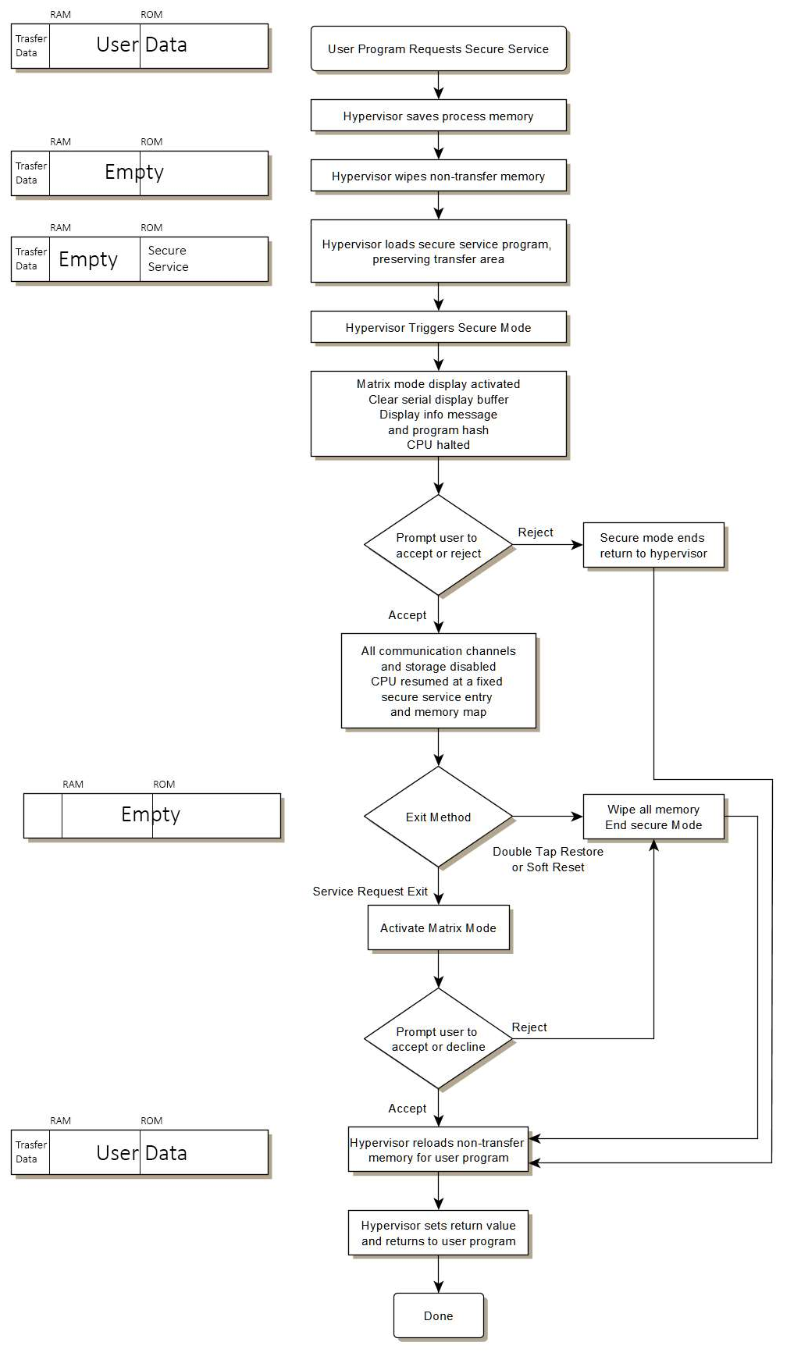
\includegraphics[width=\linewidth]{timkirby}
  \caption{The secure compartment frame work provided by Tim Kirby's thesis "Design and Development of a Secure Compartmentalised 8-bit Architecture".}
  \label{fig:timkirby}
\end{figure}

%----------------------------------------------------------------------------------------
%	SECTION 2
%----------------------------------------------------------------------------------------

\section{Initial Issues}

\label{Ch6 Sec2}

As the secure compartments were entirely separate from the matrix mode corrections and during the timea major update for another section of the phone was finished, a new branch of the project was created. Switching to this new branch resulted in overhead issues that needed to be solved in order for the project to procceed further.

%-----------------------------------
%	SUBSECTION 1
%-----------------------------------
\subsection{Repairing the Branch}

\label{Ch6 Sec2 Sub1}

As a new section of the project was being worked on the by other developers in isolation from the changes I had made, many of the fixes I had implemented had to be redone.\\
The timing fixes done to possibly correct the matrix mode issue were all removed, including the generation of the timing reports, these were reimplemented. The implementation was identical to that described in section \ref{Ch5 Sec1 Sub2} of chapter \ref{Chapter 5}.\\
All of the letterboxing changes were lost, so, as seen in section \ref{Ch5 Sec2} of chapter \ref{Chapter 5}, the erasing of the second character set was done one gains and the letterbox signal was one again used to limit the output of matrix mode.\\
The revolving line issue due to discrepancies in line length returned as was fixed as described in section \ref{Ch5 Sec3 Sub1} of chapter \ref{Chapter 5}.\\

In addition to the minor issues, matrix mode was not behaving as intended again. When attempting to enter or exit matrix mode with the tab + C= key combination, the key combination would be read and re-read rapidly and continuously. This made entering and exiting matrix mode unreliable as it was up to luck whether the key combination was scanned an odd or even amount of times to determine if the state was toggled. Tracing the matrix mode hypervisor trap from the CPU to the io mapper shows, as seen in figure \ref{fig:mmlatch}, there are latching and unlatching conditions for the matrix mode hypervisor trap. When monitoring the ascii\_key\_valid and ef\_latch signals via oscilloscope, the cause of the issue was clear. The ascii\_key\_valid signal was not a latching signal, and thus, it would only be high for a single clock cycle. As seen in the logic in figure \ref{fig:mmlatch}, this would cause the latch signal to pulse simillarly, allowing the matrix mode hyper trap to be triggered every second clock cycle. A quick solution to this issue, as seen in figure \ref{fig:traptimeout} was written by Dr. Gardner-Stephen in the form of a timeout clock that blocks repeated instances of tab + C= from triggering the matrix mode hypervisor trap.

\begin{figure}
  \centering
  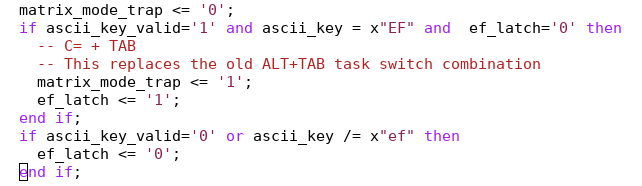
\includegraphics[width=\linewidth]{mmlatch}
  \caption{The matrix mode hypervisor trap latch.}
  \label{fig:mmlatch}
\end{figure}

\begin{figure}
  \centering
  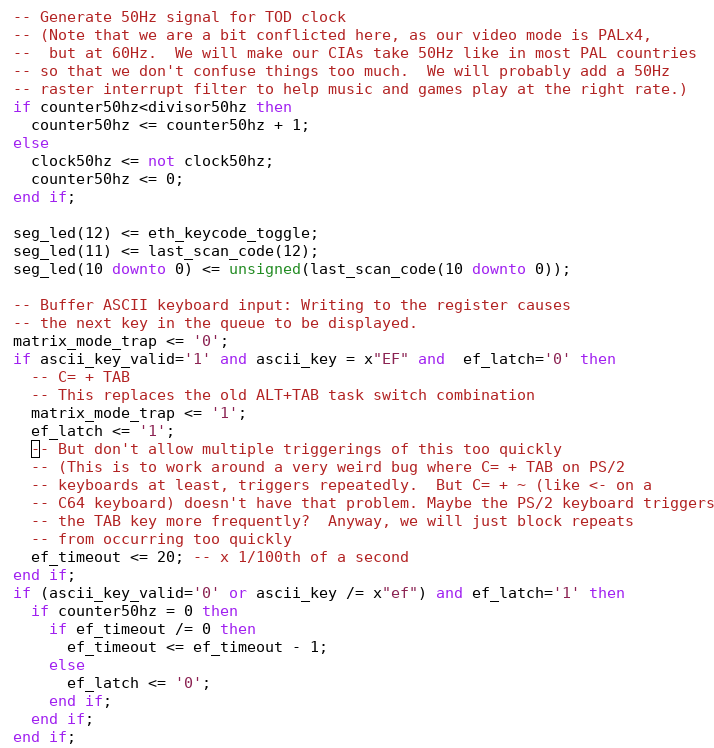
\includegraphics[width=\linewidth]{traptimeout}
  \caption{The matrix mode hypervisor trap latch with the new timeout period to prevent constant triggering.}
  \label{fig:traptimeout}
\end{figure}

%-----------------------------------
%	SUBSECTION 2
%-----------------------------------
\subsection{SD Card Restoration}

\label{Ch6 Sec2 Sub2}



Stuff about fixing the SD card

Debugging.

In order to debug the SD controller monitor load was modified.

To push things to a register S<Address> <Number>
To read a register m<Address> 
The SD control address = ffd3680
t1 = pause the CPU
t0 = Run CPU
r = view CPU status

For the ffd3680 register:
0 = Reset
1 = end reset
2 = read

It is believed that the deselect state in the sdcard.vhdl was causing the read errors for the sdhc. Look into the SDSC card deselect protocols to determine the difference between the two.

When attempting to format the SDSC card and error occur ed after the read of sector 76000000. This is believed to be the final sector. This error does not occur when reading from the sdhc card.

%----------------------------------------------------------------------------------------
%	SECTION 3
%----------------------------------------------------------------------------------------

\section{}

\label{Ch6 Sec3}

